\chapter{基础知识}

本章节介绍了本文的技术路线所使用到的一些基础知识概念和密码学工具,包括全同态加密方案 CKKS 的相关背景及其功能、椭圆曲线签名算法 ECDSA 等。

\section{全同态加密方案 CKKS}

% FIXME:摆了
\subsection{R-LWE问题}

LWE(Learning with errors) 问题是一个机器学习领域中的怀疑难解问题,由 Regev 等人提出\cite{10.1145/1568318.1568324},该问题的困难性亦被应用于公钥密码学领域。简单地说,LWE 问题是一种通过向秘密值向量引入噪声来隐藏秘密值向量的方法。

% TODO: 考虑插入学术定义

R-LWE (Ring-LWE)问题由 LWE 问题衍生,将 LWE 问题拓展至多项式环上。该问题被认为是抗量子计算的。基于 R-LWE 问题已有许多应用被提出,如密钥交换算法\cite{cryptoeprint:2012/688}和数字签名算法\cite{cryptoeprint:2011/537}。

% TODO: 也考虑插入学术定义

% 不太需要改
\subsection{CKKS 方案} \label{sec:CKKS_Review}

CKKS(Cheon-Kim-Kim-Song) 方案,又称为 HEAAN(Homomorphic Encryption for Arithmetic of Approximate Numbers),是一种允许对全体复数向量域 $\mathbb{C}^{N/2}$ 进行同态运算的全同态加密方案。其安全性来源于 R-LWE 问题的决策版本。该方案的主要特点在于以一定误差为代价,允许对复数值向量进行计算。这一关键特性意味着其突破了先前提出的同态加密方案只能对整数进行运算的限制,对于许多实际应用来说非常重要。目前 CKKS 已经集成至诸多流行的密码学库,包括 SEAL、OpenFHE 和 Lattigo 等\cite{sealcrypto,OpenFHE,Mouchet2020LattigoAM},并受到来自开源社区的优化和维护。

与以往同态加密方案将噪声空间和明文空间分开的设计不同,CKKS 方案将噪声视为明文的一部分,而噪声一方面来源于基于 R-LWE 的加密方案中为保证安全性而人为加入的误差,另一方面也来源于近似计算中的舍入误差。密文解密后不能将明文中的噪声去除,只能以预定的精度 $\Delta$ 输出明文的近似值。\cite{CKKS_optimize}

CKKS 方案由首尔大学的 Cheon 等人在 ASIACRYPT17 上首次提出\cite{cryptoeprint:2016/421},此时其属于层级全同态加密,即只支持在预定层级内进行密文之间的同态乘法,当层级降低至 0 后,密文之间的同态乘法将不再可用。随后在 2018 年 Cheon 等人提出了 CKKS 方案的自举方法\cite{cryptoeprint:2018/153},允许刷新密文的层级。该成果将该方案拓展至全同态加密。同一年晚些时候,Cheon 等人提出了 CKKS 方案的余数系统变种,极大地提升了原方案的性能。\cite{cryptoeprint:2018/931}此外,亦有实验性的使用多项式近似对两个密文进行比较的算法被提出\cite{cryptoeprint:2019/417,cryptoeprint:2019/1234,cryptoeprint:2020/834}。

CKKS 方案包含以下的核心函数和算法:

\begin{itemize}
    \item $KeyGen(\lambda) \rightarrow sk, pk, evk$:密钥生成算法,输入安全参数 $\lambda$,输出公钥 $pk$ 和私钥 $sk$,以及评估密钥 $evk$。
    \item $Ecd(z; \Delta) \rightarrow m$:对消息进行编码的算法,输入一个复向量 $z \in \mathbb{Z}^{N/2}$,输出编码后的明文 $m \in R_q = \mathbb{Z}_q[X]/(X^N+1)$;其中 $m$ 为该明文编码后对应的多项式,$\Delta$ 为编码的精度,$N$ 为该向量的最大长度。
    \item $Dcd(m; \Delta) \rightarrow z$ :将上述编码后的明文解码为复向量的算法,输入编码后的明文 $m$,输出解码后的复向量 $z$。
    \item $Enc_{pk}(m) \rightarrow ct$ :使用公钥 $pk$ 对明文 $m$ 进行加密,输出密文 $ct = (c_0(X),c_1(X)) \in R_Q^2, R_Q = Z_Q[X]/(X^n + 1)$。
    \item $Dec_{sk}(ct) \rightarrow m'$ :使用私钥 $sk$ 对密文 $ct$ 进行解密,输出明文 $m'$
    \item $Add(ct_1, ct_2)$ :对密文进行加法运算的算法,输入两个密文 $ct_1$ 和 $ct_2$,输出加法运算后的密文 $ct_{add} = ct_1 + ct_2 = Enc_{pk}(m_1 + m_2)$。
    \item $Mult_{evk}(ct_1, ct_2) = ct_1 \cdot ct_2$:对密文进行乘法运算,输入两个密文 $ct_1$ 和 $ct_2$,输出乘法运算后的密文 $ct_{mult} = ct_1 \cdot ct_2 = Enc_{pk}(m_1 \cdot m_2)$。
\end{itemize}

此外也包括以下的辅助函数:

\begin{itemize}
    \item $Rescale(ct, r) \rightarrow ct'$:即密文的重缩放过程。输入密文 $ct$ 和重缩放的精度 $r$,输出重缩放后的密文 $ct'$,其中 $ct'$ 具有更小的模数 $q' = q \cdot r^{-1}$。重缩放操作作为一种有效的密文噪声控制手段,在 CKKS 方案中起到了关键作用,有效地将同态乘法带来的噪声增长速率从指数级控制到线性级。
    \item $Rotate_{evk}(ct, k) \rightarrow ct'$:密文的旋转操作。输入密文 $ct$ 和旋转的位数 $k$,输出旋转后的密文 $ct'$。
\end{itemize}

得益于 R-LWE 问题允许对密文的密钥进行转换\cite{brakerski2014leveled},CKKS 加密方案亦适用于以下重加密方法:

\begin{itemize}
    \item $GenSwk(sk_1, sk_2) \rightarrow swk$:以私钥 $sk_1$ 和 $sk_2$ 为输入,输出用于进行密钥转换的重加密密钥 $swk$。
    \item $SwitchKey_{swk}(ct_{pk_1}) \rightarrow ct_{pk_2}$:该函数将密文 $ct_{pk_1}$ 转换为 $pk_2$ 对应的密文 $ct_{pk_2}$。
\end{itemize}

在一些库实现中,如 Lattigo,也用到了以下的扩展函数,后文亦会对其进行简要说明。


\begin{itemize}
    \item $MultByConst(ct, const) = ct'$:对密文 $ct$ 所对应的消息向量 $m = [m_1, m_2, \dots]$ 乘上一个明文常数 $const$,得到 $ct' = Enc(m')$,其中 $m' = const \cdot m  = [const \ m_1, const \cdot m_2, \dots]$。
    \item $AddConst(ct, const) = ct'$:对密文 $ct$ 所对应的消息向量 $m = [m_1, m_2, \dots]$ 的每一个元素,与明文常数 $const$ 进行相加,得到 $ct' = Enc(m')$,其中 $m' = [const + m_1, const + m_2, \dots]$。
\end{itemize}

下图\cite{ckksIntroduct} \ref*{Fig:CKKS}描述了 CKKS 方案的工作生命周期:

\begin{figure}[ht]
    \centering
    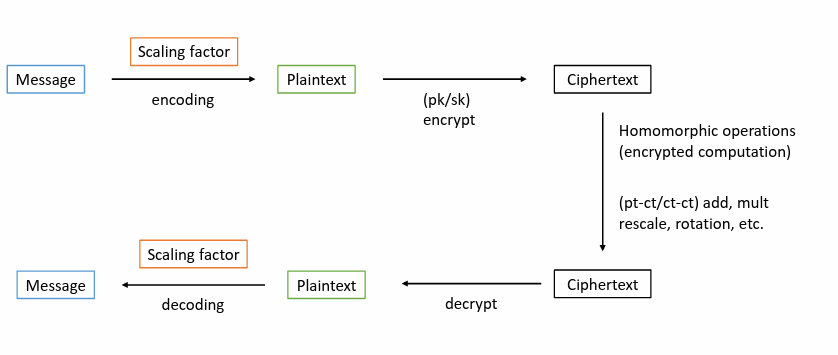
\includegraphics[width=\linewidth]{./Figures/CKKS_Diagram.png}
    \caption{CKKS 方案工作示意图}\label{Fig:CKKS}
\end{figure}

\section{数字签名算法 ECDSA} \label{sec:ecdsa}

数字签名是一种公钥密码学技术,于 1976 年被首次提出\cite{1055638}。其原理为对于某一信息,该算法可以使用私钥生成该信息的一个签名,并且可以被公钥验证。若验证不通过,则认为该信息被受到修改不是原信息;反之则可以确认该签名是由私钥持有者生成的,即该信息是由私钥持有者发送的。数字签名的应用领域包括防止消息纂改,以及验证某一消息是否真实地由某人发出。

本文方案使用了椭圆曲线数字签名算法,即 ECDSA(Elliptic Curve Digital Signature Algorithm)。该算法由 DSA 签名算法与椭圆曲线密码体制结合而成,并逐渐成为 ANSI\footnote{American National Standards Institute,美国国家标准学会}、IEEE\footnote{Institute of Electrical and Electronics Engineers,电气电子工程师学会}、ISO\footnote{International Organization for Standardization,国际标准化组织} 和 NIST\footnote{National Institute of Standards and Technology,美国国家标准技术研究所} 标准\cite{ecdsa_blockchain}。基于椭圆曲线的密码学算法被认为是难以攻击的。NIST 和 SECG 等组织提供了很多的预制的标准化曲线,且已经在业界被广泛使用,如 NIST 提供的 P-256 等标准曲线\footnote{也被称为 secp256r1}、Brainpool 曲线,以及 Curve 25519\cite{10.1007/11745853_14} 等。下面将对 ECDSA 的签名流程进行简要介绍。

\begin{enumerate}
    \item 初始化:选择椭圆曲线 $E$,得到公共安全参数 $\{a, b, p, N, G\}$。其中椭圆曲线如公式\eqref{eq:elliptic}所示,$G$ 为生成元,$N$ 为椭圆曲线上的点数量。
    \begin{equation} \label{eq:elliptic} 
        E: y^2 = (x^3 + a \times x + b) mod p
    \end{equation}
    \item 公私钥生成:选择随机整数 $sk$ 作为私钥,计算\eqref{eq:elliptic_pk}得到公钥 $pk$,其中 $\times$ 是一个单向陷门函数,通过公钥反推私钥是困难的。
    \begin{equation} \label{eq:elliptic_pk}
        pk = sk \times G
    \end{equation}
    \item 签名:对消息 $m$ 生成其摘要 $h = Hash(m)$,通过公式\eqref{eq:elliptic_sign_1}和\eqref{eq:elliptic_sign_2}计算签名 $Sig = (R, S)$,其中 $k$ 为一随机数。
    \begin{equation} \label{eq:elliptic_sign_1}
        P(x_1, y_1) = k \times G, R = x_1 mod N
    \end{equation}
    \begin{equation} \label{eq:elliptic_sign_2}
        S = k^{-1} (h + sk \times R) mod p
    \end{equation}
    \item 验证:挑战者接收到消息 $m$ 和签名 $(R, S)$,在生成摘要后通过式子\eqref{eq:elliptic_verify_1}计算验证签名,若式子\eqref{eq:elliptic_verify_2}成立,则签名被接受
    \begin{equation} \label{eq:elliptic_verify_1}
        P(x_1, y_1) = S^{-1} \times h \times G + S \times R \times pk (mod N)
    \end{equation}
    \begin{equation} \label{eq:elliptic_verify_2}
        x_1 = R (mod N)
    \end{equation}
\end{enumerate}

将上面的流程简化,可以得到以下方法:

\begin{itemize}
    \item $KeyGen(\lambda) \rightarrow sk, pk$:输入安全参数 $\lambda$,输出一对随机生成的私钥 $sk$ 和公钥 $pk$。
    \item $Sign(m, sk) \rightarrow sig$:使用私钥 $sk$ 对消息 $m$ 进行签名,输出签名 $sig$。
    \item $Verify(m, pk, sig) \rightarrow bool$:使用公钥 $pk$ 对签名 $sig$ 进行验证,输出验证结果 $bool$。
\end{itemize}

\section{本章小结}

本章首先介绍了同态加密和全同态加密,及其发展历程。然后,本章重点介绍了本文所使用的全同态加密方案 CKKS,包括其基于的困难问题,CKKS 方案的特点,以及该加密方案包含的主要函数等。本章也对椭圆曲线签名算法等涉及到的其他密码学工具,进行了简要的介绍。本章内容是后文的基础,后续对交易方案的构建都在本章基础之上完成。
